\chapter{Variabili Aleatorie}

\begin{figure}[H]
	\centering
	\caption{Tipi di variabili casuali}
	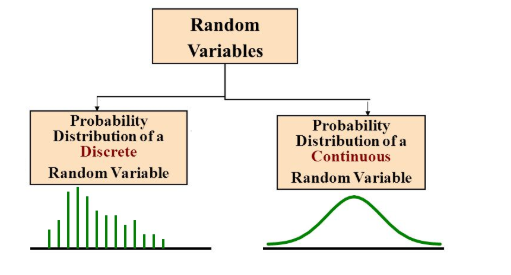
\includegraphics[]{varrandom}
\end{figure}

\section{Variabili Aleatorie Discrete}

\begin{defn}
	Una variabile aleatoria (casuale o stocastica) discreta è una variabile che può assumere diversi valori in dipendenza da qualche fenomeno casuale.
	Il risultato del lancio di un dado, ad esempio, è una variabile aleatoria discreta.
	
	Prendiamo uno \textbf{spazio probabilizzabile} $ (\Omega, F) $ e una variabile aleatoria discreta $ X : \Omega \to \R $, che è una funzione continua non surgettiva. I valori di $ X $ devono essere un sottoinsieme finito di $ \R $ ovvero $ \{a_1, \dots, a_k\} $.
	Vogliamo anche che $ \forall j \in [1, k] $ sia vero $ X^{-1}(a_j) = \{ \omega \in \Omega, X(\omega) = a_j\} \in F $. Utilizziamo la funzione inversa per ottenere gli elementi di $ \Omega $ su cui possiamo definire la probabilità.
	
	Con la probabilità di tutti gli eventi definisco la densità di probabilità. Nello spazio probabilizzato $ (\Omega, F, \mathcal{P}) $ la probabilità che la variabile aleatoria assuma il valore $ a_j $ sarà $ p_j = \p{X = a_j} = \p{X^{-1}(a_j)} $, che viene detta densità di probabilità. Varranno quindi le seguenti proprietà
	
	\begin{enumerate}
		\item $ \forall j \ldotp X^{-1} (a_j) $ sono tutti insiemi disgiunti.
		\item Essi coprono tutto $ \Omega $
	\end{enumerate}
	Vale che $ \sum_{j=1}^{k} p_j = 1 $. Poiché:
	
	\begin{equation*}
		1 = \p{\Omega} = \p{\bigcup_{j} X^{-1}(a_j)} = \sum_{j} \p{X^{-1}(a_j)}
	\end{equation*}
	
	Sia $ X : \Omega \to \{ a_1, \dots, a_k \} $ una variabile aleatoria, e sia la densità di probabilità $ p_j \geq 0 $ e anche  $ \sum_{j=1}^{k} p_j = 1 $, allora $ \p{X = a_j} = p_j $.
	
	Preso uno spazio probabilizzabile $ (\Omega, F) $ e una variabile aleatoria $ X : \Omega \to \{ a_1, \dots, a_k \} $, supponendo che i numeri $ a_j $ siano ordinati, sia $ p_j $ la densità di probabilità, come posso ricostruire, ad esempio $ \p{x \leq a_3} $?
	
	\begin{equation*}
		\p{X \leq a_3} = \p{(X=a_1) \cup (X=a_2) \cup (X=a_3)} = \p{X = a_1} + \p{X = a_2} + \p{X = a_3}
	\end{equation*}
	
\end{defn}

\begin{exmp}
	Voglio contare quanti 6 escono in 10 lanci di dadi.
	
	Sia $ \Omega = \{ (1, 2, 3, 4, 5, 6)\}^{10} $, ovvero tutte le possibili parole di 10 elementi composte dai numeri da 1 a 6. Ad ogni lancio, ho $ \frac{1}{6} $ di probabilità di ottenere 6 e $ \frac{5}{6} $ di ottenere gli altri numeri. Definiamo la variabile aleatoria $ X : \Omega \to \{ 0, 1, 2, \dots, 9, 10 \} $ come il conteggio dei risultati dei lanci dove ottengo 6. Qual'è la probabilità di ottenere 3 lanci dove ho fatto 6?
	
	\begin{equation*}
		\p{X = 3} = \binom{10}{3} \left(\dfrac{1}{6}\right)^3 \left(\dfrac{5}{6}\right)^7 
	\end{equation*}
\end{exmp}

\section{Leggi su Variabili Aleatorie}

\begin{defn}
	\textbf{Legge di Bernoulli:}
\end{defn}
Faccio un esperimento, il risultato positivo ha probabilità $ p $, mentre il risultato negativo ha probabilità $ 1 - p $. Sia lo spazio $ \Omega = \begin{cases}
\text{successo} \to 1 \\
\text{insuccesso} \to 0
\end{cases} $. Una variabile aleatoria Bernoulliana è definita come $ X : \Omega \to \begin{cases}
p_1 = p \\ p_0 = 1 - p
\end{cases} $

\begin{defn}
	\textbf{Legge Binomiale} 
	Sia $ k $ il conteggio dei successi di $ n $ esperimenti, abbiamo quindi che $ B(n,p) = X_i\{(0,1)\}^n \to \{0, \dots, n\} $. Abbiamo che la densità di probabilità Binomiale $ p_k = \p{X=k} = \binom{n}{k} p^k(1-p)^{n-k} $.
	
	$ p_k $ è una densità? Sappiamo che $ p_k \geq 0 $ e sappiamo che $ 1 = \sum_{k} p_k $, con il binomio di Newton possiamo dimostrare che $ (a+b)^n = \sum_{k=0}^{n} \binom{n}{k} a^k b^{n-k} $. Proseguendo, abbiamo che 
	
	\begin{equation*}
		\sum_{k} p_k = \sum_{k=0}^{n} \binom{n}{k} p^k (1-p)^{n-k} = (p+(1-p)^n) = 1^n = 1
	\end{equation*}
\end{defn}

\begin{defn}
	\textbf{Somma di Variabili Aleatorie}
	Lancio due dadi, uno rosso e uno nero, avremo quindi $ \Omega = \{R, N\} = \{(1,6)\}^2 $. Definisco due variabili aleatorie, $ X $ per il dado rosso dove $ X : (R, N) \to R $ e la variabile $ Y : (R, N) \to N $. La densità per $ X $ sarà $ p_j = \frac{1}{6} \forall j $ mentre la densità per $ Y $ sarà $ q_j = \frac{1}{6} \forall j $
	Avremo che $ Z = X + Y $ conta la somma dei dadi.
\end{defn}

\begin{exmp}
	Calcolare la densità di $ Z $
	
	In questo caso $ X, Y $ sono indipendenti, quindi avremo la densità di $ Z $ detta $ t_Z $.
	
	\begin{equation*}
	\forall n \in [2, 12] .  \left( \p{Z = n} = \sum_{i=1}^{n-1} \p{X = i} \cdot \p{Y = n - i} \right)
	\end{equation*}
	
	\begin{table}[H]
		\centering
		\caption{Distribuzione discreta della somma del lancio di due dadi.}
		\label{tab:distribdice1}
		\begin{tabular}{|l|l|l|l|l|l|l|l|l|l|l|l|}
			\hline
			$ X + Y $     & 2        & 3        & 4        & 5        & 6        & 7        & 8        & 9        & 10       & 11       & 12       \\ \hline
			$ p_j + q_j $ & $ 1/36 $ & $ 2/36 $ & $ 3/36 $ & $ 4/36 $ & $ 5/36 $ & $ 6/36 $ & $ 5/36 $ & $ 4/36 $ & $ 3/36 $ & $ 2/36 $ & $ 1/36 $ \\ \hline
		\end{tabular}
	\end{table}
	
	\begin{figure}[H]
		\centering
		\caption{Distribuzione della somma del lancio di due dadi}
		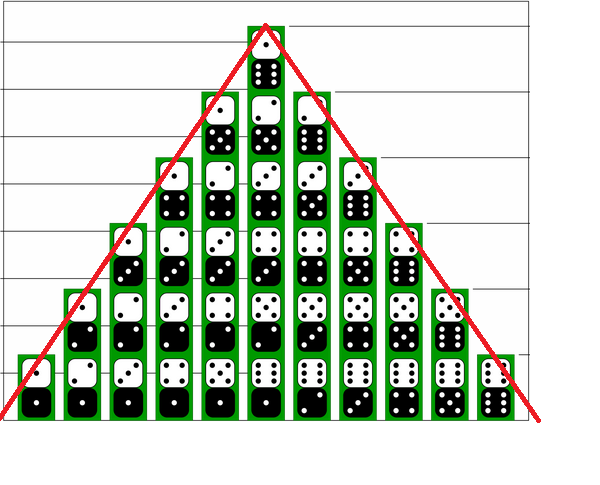
\includegraphics[]{binomdadi}
	\end{figure}
\end{exmp}

\begin{exmp}
	Calcolare $ \p{4 \leq Z \leq 6} $
	
	\begin{equation*}
	\p{4 \leq Z \leq 6} = \p{Z = 4} + \p{Z = 5} + \p{Z = 6} = \dfrac{3}{36} + \dfrac{4}{36} + \dfrac{5}{36} = \dfrac{12}{36} = \dfrac{1}{3}
	\end{equation*}
\end{exmp}		


\begin{defn}
	\textbf{Indipendenza di variabili aleatorie}
	Due variabili aleatorie $ X_1, X_2 $ sono indipendenti se $ \forall I_1, I_2, \subseteq \R $ intervalli o semirette si ha che 
	
	\begin{equation*}
	\left( \p{X_1 \in I_1} \cap \p{X_2 \in I_2} \right) = \p{X_1 \in I_1} - \p{X_2 \in I_2}
	\end{equation*}
	
	Nell'esempio di prima $ X, Z $ e $ Y,Z $ sono dipendenti perché dati $ I_1 = [1,2], I_2 = [3,4] $ allora si ha che $ \p{X\in I_1} = \p{X=1,2} = \dfrac{1}{3} $ e si ha anche $ \p{Z \in I_2} = \p{2 = 3,4} = \dfrac{5}{36} $. Ne otteniamo che:
	
	% TODO fix erratum
	
	\begin{equation*}
	\p{(X \in I_1) \cap (Z = 3,4)} = \p{X = 1,2, Z = 3,4} = \dfrac{4}{12}
	\end{equation*}
		
\end{defn}

\begin{defn}
	\textbf{Variabili Aleatorie Congiunte}
	Due variabili aleatorie $ X,Y : \Omega \to \R $ discrete sono congiunte quando si può calcolare $ \p{X = m \cap Y = n} = p_{n,m} $, ovvero una densità di probabilità $ \{ p_{n,m} \}_{n,m} $ con $ (p_{n,m} \geq 0 ) \land (\sum_{n,m} p_{n,m} = 1) $.
	
	Sapendo $ p_{n,m} $ ricavo tutti i $ \p{X=m} = p_m $ e $ \p{Y = n} = q_n $ con
	
	\begin{equation*}
	\begin{aligned}
	\p{X=m} = \p{X = m \cap \left\{ \bigcup_{n} Y=n \right\}} \\ 
	= \sum_{n} \p{X=m,Y=n} = \sum_n p_{n,m} = p_m \\
	\p{Y=n} = \sum_{m} p_{n,m} = q_n
	\end{aligned}
	\end{equation*}
	
	Non si può ricostruire dalle due probabilità la variabile aleatoria congiunta. Ad esempio, conoscendo $ p_n,q_n $ cerco $ p_n,m  = \p{X = m \cap Y = n} = \p{X = m | Y = n} \cdot \p{Y=n} $. Se $ X,Y $ sono indipendenti allora $ P(X=m \mid Y=n) = \p{X=m} $ e vale il prodotto $ p_{m,n} = p_n \cdot p_m $.
	
	
	\begin{equation*}
	\sum_{m}\sum_{n} p_{n,m} = \sum_{m}\sum_{n} p_n \cdot q_n = \left( \sum_{m} p_m \right) \left( \sum_{n} q_m \right) = 1 
	\end{equation*}
\end{defn}


\begin{defn}
	\textbf{Formula di Convoluzione}
	
	Tornando alla somma di due variabili aleatorie discrete, dati $ X,Y $ indipendenti e $ Z = X + Y $, con $ X,Y : \Omega \to \N $, dobbiamo calcolare $ \p{Z = n} $ e la densità di probabilità discreta $ \left\{Z = n\right\} $
	
	\begin{equation*}
	\begin{aligned}
	\left\{Z = n\right\} = \bigcup_{i=0}^{n} \left\{X = 1 \cap Y = n - i \right\} \\
	\p{z=n} = \sum_{i} \p{X = i \cap Y = n-1} = \sum_{i = n}^{n} \p{X=i} \cdot \p{Y=n-i}
	\end{aligned} 
	\end{equation*}
\end{defn}

\begin{thm}
	\textbf{Rapporto fra Bernoulli e Binomiale}
	
	Sommando $ n $ esperimenti di $ p $ dove conto i successi ottengo la binomiale $ B(n,p) $, quindi $ \sum_{i=1}^{n} \text{Bern}_i(p) = B(n,p) $
	
	\begin{proof}
		Caso base, per $ n = 1 \implies B(1,p) = \text{Bern}(p)$. Come passo induttivo abbiamo 
		
		\begin{equation*}
		\begin{aligned}
		B(n,p) = \sum_{i=1}^{n} \text{Bern}_i(p) \implies B(n+1,p) = \sum_{i=1}^{n+1} = \text{Bern}_i(p) \\
		\sum_{i=1}^{n+1} \text{Bern}_i(p) = \left( \sum_{i=1}^{n} \text{Bern}_i(p) \right) + \text{Bern}_{n+1}(p) = B)(n,p) + \text{Bern}(p)
		\end{aligned}
		\end{equation*}
		
		Introduciamo le densità per continuare la dimostrazione
		
		\begin{equation*}
		\begin{aligned}
		\p{B(n,p) + \text{Bern}(p) = k} = \p{B(n,p) = k \cap \text{Bern}(p) = 0} + \p{B(n,p) = k-1 \cap \text{Bern}(p) = 1} \\
		= \binom{n}{k-1}p^{k-1}(1-p)^{n-k+1} \cdot p + \binom{n}{k}p^k(1-p)^{n-k} \cdot  (1-p) \\
		= \left[\binom{n}{k-1}\binom{n}{k}\right] p^k (1-p)^{n-k+1} = \binom{n+1}{k} p^k (1-p)^{n+1-k} = \p{B(n+1,p) = k}
		\end{aligned}
		\end{equation*}
	\end{proof}
	

\end{thm}


\begin{defn}
	\textbf{Variabile Geometrica}
	Data una successione di esperimenti ripetuti con probabilità di successo $ 0 \leq p \leq 1 $. Lo ripeto fino ad ottenere un successo. $ \geom(p) $ conta il numero di prove necessarie. Ovvero $ \p{\geom(p) = k} = $ la probabilità di fare k esperimenti ed avere un successo dall'ultimo. La densità di probabilità sarà $ p_k = \p{\geom(p) = k} = (1-p)^{k-1} \cdot p $ con $ p_k \geq 0 $ e anche $ \sum_{k=1}^{\infty} (1-p)^{k-1} p = p \sum_{k=1}^{\infty}(1-p)^{k-1} $, che è una serie geometrica. Sarà quindi equivalente a $ p \sum_{i=0}^{n} (1-p)^i = \dfrac{p}{1-(1-p)} = 1$
	
	
	Osservazione: consideriamo la serie geometrica $ \sum_{i=0}^{\infty} q^i $.
	Sappiamo che $ (1-q) \sum_{i=0}^{\infty} q^i = 1 $ perché $ (1-q)(1+q+q^2+q^3\dots) $ = $( 1 - q + q - q^2 + q^2 + \dots )$, semplificando i termini rimane 1.
	
	Una variabile geometrica \textbf{non ha memoria}, l'esperimento numero $ n $ ha la stessa probabilità degli altri esperimenti:
	
	\begin{equation*}
	\begin{aligned}
	\p{\geom(p) = n+m | \geom(p) > n} = \p{\geom(p) = m} \\
	= \dfrac{\p{\geom(p) = m + n \cap \geom(p) > n}}{\p{\geom(p) > n}} = \dfrac{\p{\geom(p) = m+n}}{\p{\geom(p) > n}}\\ 
	= \dfrac{(1-p)^{m+n-1} \cdot p}{(1-p)^n} = \p{\geom(p) = m} \\
	\end{aligned}
	\end{equation*}
	
	Si può dimostrare sapendo che $ \forall m . \p{\geom(p) = n+m \cap \p{\geom} > n} = \p{\geom(p) = m+n} $
	
\end{defn}

\begin{defn}
	\textbf{Variabili Ipergeometriche}
	
	Siano dati $ r $ sfere rosse, $ b $ sfere bianche, $ n $ estrazioni senza reimbussolamento, $ k = $ numero di sfere rosse estratte, $ H(b+r, r, n) $ conta il numero di sfere rosse estratte dopo n tentativi. È detta variabile ipergeometrica. Sappiamo che $ (0 < n \leq b + r) \land (k \leq n)  \land (k \leq r) \land (n-k \leq b) $.
	
	Definiamo la densità di probabilità
	\begin{equation*}
	\p{H(b+r, r, n) = k} = \dfrac{\binom{r}{k} \binom{b}{n-k}}{\binom{b+r}{n}}
	\end{equation*}
\end{defn}


\begin{defn}
	\textbf{Binomiale Negativa (o di Pascal)}
	Sia data una Bernoulliana di parametro $ p $. Ripetiamo l'esperimento fino a che non ho $ n $ successi. Quanti sono i fallimenti ottenuti? Sappiamo che una variabile Binomiale conta i successi, una variabile Geometrica conta i fallimenti prima del primo successo e la Binomiale Negativa (NB) conta i fallimenti prima del successo $ n $-esimo. In una Binomiale Negativa non conta l'ordine degli esperimenti (tranne l'ultimo risultato). Le prove totali prima di avere $ n $ successi sono $ n+\text{NB} $. Sapendo che per avere $ n $ successi e $ k $ fallimenti, la probabilità di una Binomiale Negativa è definita come 
	
	\begin{equation*}
	\p{\nb{n, p} = k} = p^n(1-p)^k
	\end{equation*}
\end{defn}

\begin{exmp}
	Lancio una moneta fino ad ottenere 3 croci (non consecutive). Qual'è la probabilità di aver fatto esattamente 2 risultati testa? $ \p{\nb{3, \frac{1}{2}} = 2} = \binom{3+2-1}{2} \left(\frac{1}{2}\right)^3 \left(\frac{1}{2}\right)^2 = \frac{3}{16} $. 
	
	La probabilità di ottenere almeno un risultato testa è $ \p{\nb{3, \frac{1}{2}} = 0} = 1 - \frac{1}{8} = \frac{7}{8} $
\end{exmp} 

\section{Valore Atteso}

\begin{defn}
	\textbf{Media Pesata, Speranza o Valore Atteso}
	Consideriamo di voler calcolare la media pesata dei voti degli esami universitari. La media sarà per ogni esame $ i $:
	\begin{equation*}
	\sum_{i} \dfrac{(\text{voto})_i \cdot (\text{crediti})_i }{\sum_{i} \text{crediti}} = \sum_{i} (\text{voto})_i \cdot (\text{peso})_i
	\end{equation*}
	
	Definiamo $ X $ variabile aleatoria discreta $ X \subseteq \R $. La media di $ X $ è detta \textbf{speranza} o \textbf{valore atteso} e si denota con
	
	\begin{equation*}
	\E{X} = \sum_{k} k \cdot \p{X = k} = \sum_{k} k \cdot p_k
	\end{equation*}
	
	Per calcolare la media di una funzione $ f : \R \to \R $:
	
	\begin{equation*}
	\E{f(X)} = \sum_{k} f(k) \cdot p_k
	\end{equation*}
	
	\textbf{Osservazione} $\sum_{k} p_k = 1 $ \textbf{non implica che} $ \sum_{k} k p_k $ sia convergente. Se non converge ad un numero allora la variabile non ha media. Se la variabile assume solo valori positivi allora
	
	\begin{equation*}
	\E{X} = \sum_{k>0} \p{X > k} = \sum_{k>0} (\p{X = k+1} + \p{X = k+2} + \dots)
	\end{equation*}
	
\end{defn}

\begin{defn}
	Speranza di una Binomiale $ B(n,p) $. La distribuzione $ p_k = \binom{n}{k}p^k(1-p)^{n-k}  \forall k \in [0,n] $. Abbiamo che $ kp_k = k \binom{n}{k}p^k (1-p)^{n-k} = n \binom{n-1}{k-1} p^k(1-p)^{n-k} $. Definiamo $ h = k-1 $.
	
	\begin{equation*}
		\begin{aligned}
			\E{B(n,p)} = \sum_{k=1}^{n} kp_k = \sum_{k=1}^{n} n \binom{n-1}{k-1} p^k(1-p)^{n-k} \\
			= np \sum_{k} \binom{n-1}{k-1}p^{k-1}(1-p)^{n-k} \\
			= np \sum_{h=0}^{n-1} \binom{n-1}{h} p^h(1-p)^{(n-1) - h } \\
			= np(p+(1-p))^{n-1} = np
		\end{aligned}
	\end{equation*}

\end{defn}

\begin{defn}
	Speranza di una variabile geometrica $ \geom(p) $, che conta il numero di successi prima di un successo:
	\begin{equation*}
	\E{\geom(p)} = \sum_{k=0}^{\infty} k(1-p)^k p = \sum_{k}\p{\geom(p) > k}
	\end{equation*}
	Prendiamo in caso 
	\begin{equation*}
		\sum_{k}\p{\geom(p) > k} = \sum_{h=k+1}^{\infty} (1-p)^(h-1)p = \sum_{k}(1-p)^k = \dfrac{1}{1-(1-p)} = \dfrac{1}{p}
	\end{equation*}
\end{defn}


\begin{exmp}
	Scommetto. Pago 1 euro. Lancio 3 dadi e guadagno 1 euro ogni 6 che esce.
	Rappresento il guadagno con una variabile binomiale $ X = B(3,1/6) - 1$. Abbiamo che $ \E{X} = \E{B(3,1/6)} - 1 = 3 \cdot 1/6 - 1 = -1/2$
\end{exmp}
		

\begin{defn}
	\textbf{Distribuzione di Poisson}
	Nel caso di una variabile binomiale conosco $ p $ e $ n $ (numero esperimenti).
	In una distribuzione di Poisson si conosce una media $ \mu $ di successi in un intervallo di osservazione.
	Definiamo un intervallo $ \tau $, suddiviso in $ n $ sottointervalli. Abbiamo $ \mu $ successi. Se $ n $ è grande abbastanza tale che in ogni intervallo avviene 1 evento, generati da $ n $ esperimenti indipendenti allora $ \mu = \E{B(n,p)} = np$. Ne segue che:
	
	\begin{equation*}
	\begin{aligned}
	p = \dfrac{\mu}{n} 
	\p{B(n,p) = k} = \binom{n}{k}p^k(1-p)^{n-k} = \binom{n}{k} \left(\dfrac{\mu}{n}\right)^k \left(1- \dfrac{\mu}{n}\right)^{n-k} 
	= \\ \dfrac{n!}{k!(n-k)!} \dfrac{1}{n^k} \dfrac{\mu^k}{\left(1-\dfrac{\mu}{n}\right)^k} \cdot \left(1-\dfrac{\mu}{n}\right)^n  
	= \\ \dfrac{n^k \cdot \left(1-\dfrac{1}{n} \right) \cdot \left(1-\dfrac{2}{n}\right) \cdot \dots \cdot \left(1- \dfrac{k-1}{n}\right)}{k!} \cdot \dfrac{\mu^k}{\left(1-\dfrac{\mu}{n}\right)^k} \cdot \left(1-\dfrac{\mu}{n}\right)^n 
	\end{aligned}
	\end{equation*}
	
	Ne otteniamo che 
	\begin{equation}
	\p{\text{Poisson}(\mu) = k} = \dfrac{\mu^k}{k!} e^{-\mu}
	\end{equation}
	
	% TODO dimostrazione strana
\end{defn}

\begin{exmp}
	Siamo nel secolo 1800, prendiamo l'esercito di Napoleone nel reparto della cavalleria. Ogni anno 12 cavalieri muoiono per incidente a cavallo. Voglio sapere la probabilità che nel 1861 siano morti 7 cavalieri.
	\begin{equation*}
	\p{\text{anno } 1861 | \text{sono morti 7 cavalieri}}
	\end{equation*}
	Utilizziamo la distribuzione di Poisson.
	
	\begin{equation*}
	\p{\text{Poisson}(12) = 7} = \dfrac{12^7}{7}e^{-12} \approx 0.04
	\end{equation*}
	
\end{exmp}

\begin{defn}
	\textbf{Linearità della media}
	
	Siano date $ X,Y $ variabili aleatorie, $ \alpha ,\beta \in \R $. Abbiamo che
	
	\begin{equation*}
	\E{\alpha X + \beta Y} = \alpha \E{X} + \beta \E{Y}
	\end{equation*}
\end{defn}


\begin{defn}
	\textbf{Valore atteso della somma}
	
	\begin{equation}
	\begin{aligned}
	\E{X+Y} = \E{X} + \E{Y}
	\end{aligned}
	\end{equation}
	
	\begin{proof}
		\begin{equation*}
		\begin{aligned}
		\E{X+Y} = \sum_{i,j} (i+j)p_{ij} = \sum_{i,j} ip_{ij} + \sum_{i,j} jp_{ij} \\
		= \sum_i i \sum_j p_{ij} + \sum_j j \sum_i p_{ij} \\
		= \sum_i i p_i^X + \sum_j p_j^Y = \E{X} + \E{Y}
		\end{aligned}
		\end{equation*}
	\end{proof}

%	TODO fix proof
\end{defn}

\begin{defn}
	\textbf{Valore atteso del prodotto}
	Siano date $ X,Y $ variabili aleatorie \textbf{indipendenti}.
	
	\begin{equation*}
	\begin{aligned}
	\E{X \cdot Y} = \E{X} \cdot \E{Y} = \sum_{i,j} i \cdot j \cdot \p{X = i \cap Y =j} \\
	= \sum_{i,j} i \cdot j p_{ij} = \sum_{i,j} ij p_i^X p_j^Y =  \sum_{i} i p_i^X \cdot \sum p_j^Y
	\end{aligned}
	\end{equation*}
\end{defn}


\begin{defn}
	\textbf{Ordinamento}
	
	Sia $\E{X^n}$ ordinamento di ordine n.
	Dato un $ \E{f(x)} $, ad esempio $ \E{X^n} = \sum_i i^n p_i$
	Oppure ad esempio $ \E{X^2} = \sum_i i^2 \p{X = i}$. Ne segue che $ \E{X^2} \neq \left(\E{X}\right)^2$.	
\end{defn}


\begin{defn}
	\textbf{Varianza}
	
	Sia $ X $ una variabile aleatoria e $ \E{X} = \mu $ la sua media.
	La varianza di $ X $ si definisce come 
	
	\begin{equation*}
	\begin{aligned}
	\var{X} = \E{(X-\mu)^2} \\ 
	= \sum_i (i-\mu)^2 \p{X = i}
	\end{aligned}
	\end{equation*}
	
	La varianza di $ X $ è anche $ \E{X^2} - \left(\E{X}\right)^2 $
	
	\begin{proof}
		\begin{equation*}
		\begin{aligned}
		\sum_i (i-\mu)^2 p_i = \sum_i (i^2 -2i\mu + \mu^2) p_i \\
		= \sum_i i^2 p_i - 2\mu \sum_i i p_i + \mu^2 \sum_i p_i \\
		= \E{X^2} - 2\mu^2 + \mu^2 = \E{X^2} - \mu^2 \\
		= \E{X^2} - \left(\E{X}\right)^2 
		\end{aligned}
		\end{equation*}
	\end{proof}
\end{defn}



\begin{defn}
	\textbf{Disuguaglianza di Hölder}
	
	\begin{equation}
		\begin{aligned}
		\E{X \cdot Y} \leq (E[X^p])^{\frac{1}{p}} (E[Y^q])^{\frac{1}{q}} \\
		\text{con } \dfrac{1}{p} + \dfrac{1}{q} = 1
		\end{aligned}
	\end{equation}
\end{defn}


\begin{defn}
	\textbf{Disuguaglianza di Markov}
	
	\begin{equation}
		\begin{aligned}
		X \geq 0 \land a > 0 \\
		\p{X > a} < \dfrac{\E{X}}{a}
		\end{aligned}
	\end{equation}
\end{defn}

\begin{defn}
	\textbf{Disuguaglianza di Chebichev}
	
	\begin{equation*}
		\begin{aligned}
			X \geq 0 \land a > 0 \\
			\p{\abs{X - \mu} > a} \leq \dfrac{\var{X}}{a^2}
		\end{aligned}
	\end{equation*}
	
	Dimostriamo la disuguaglianza di Chebichev in quanto ci sarà utile nel resto del corso
	
	\begin{proof}
		\begin{equation*}
			\begin{aligned}
				\p{\abs{X - \mu} > a} = \sum_n \p{X = n} = \sum_{\abs{X - \mu} > n} p_n \\
				\text{se } \abs{X - \mu} > a \text{ allora } 1 < \dfrac{\abs{X - \mu}^2}{q^2} \\ \implies  \sum_{\abs{X - \mu} > n} p_n  \leq \sum_{\abs{X - \mu} > n} \dfrac{\abs{X - \mu}^2}{a^2} p_n \leq \dfrac{1}{a^2} \sum_n \abs{n - \mu}^2 p_n 
			\end{aligned}
		\end{equation*}
	\end{proof}
\end{defn}


\begin{defn}
	\textbf{$\sigma$ Deviazione Standard}
	
	Sia $ X $ variabile aleatoria. Allora abbiamo che $ \sigma(X) = \sqrt{\var{X}} $. Data $ \mu $ media di $ X $, e dati $ \alpha, \beta \in \R $ si ha allora che
	
	\begin{equation*}
		\begin{aligned}
			\var{\alpha X + \beta} = \alpha ^2 \var{X} \\
			= \E{(\alpha X + \beta)^2} - (\E{\alpha X + \beta})^2 \\
			= \E{\alpha^2 X^2 + 2 \alpha \beta X + \beta^2} - (\alpha \E{X} + \beta)^2 \\
			= \alpha^2 (\E{X^2} - (\E{X})^2) = \alpha^2 \var{X}
		\end{aligned}
	\end{equation*}
\end{defn}


\begin{defn}
	\textbf{Somma di varianza} 
	
	Siano date $ X,Y $ variabili aleatorie indipendenti $ \implies \var{X + Y} = \var{X} + \var{Y} $ 
	
	\begin{proof}
		\begin{equation*}
		\begin{aligned}
		\var(X+Y) = \E{(X+Y)^2} - (\E{X+Y})^2 \\
		= \E{X^2} - 2\E{X \cdot Y} + \E{Y^2} \\ 
		= (\E{X})^2 - 2\E{X}\E{Y} - (\E{Y})^2 \\
		= \var{X} + \var{Y} + 2(\E{XY} - \E{X}\E{Y})\\
		\text{Si ha che } 2(E[XY] - \E{X}\E{Y}) = 0 \text{ se X,Y sono indipendenti.}
		\end{aligned}
		\end{equation*}
	\end{proof}
	
\end{defn}


\begin{exmp}
	Varianza di una Bernoulliana: $ X = B(1,p) $
	\begin{equation*}
	\begin{aligned}
		\E{X} = p \\
		\E{X}^2 = p \\
		\var{X} = p-p^2 = p(1-p)
	\end{aligned}
	\end{equation*}
\end{exmp}

\begin{exmp}
	$ X = B(n,p) \implies \var{X} = nB(1,p) = np(1-p) $
\end{exmp}

\begin{exmp}
	$ X = \text{Poisson}(\lambda)  \implies  \var{\text{Poisson}(\lambda)} = \lambda $
\end{exmp}





\section{Esercizi}

\begin{exrc}
	\item Dati $ r = 10, 15 = b, 7 = n $ abbiamo che $ \p{H(25,15,7) = 3} $ è $ \dfrac{\binom{15}{3}\binom{10}{7-3}}{\binom{25}{7}} $
	
	\item Ho una scatola con 12 lampadine, 4 di esse sono fulminate. Ne prendo 2. La probabilità che siano entrambe funzionanti è $ \p{H(12, 4, 2) = 0} = \dfrac{\binom{4}{0}\binom{8}{2}}{\binom{12}{2}} $
	
	\item Ho una moneta truccata. La probabilità che esca testa è $ P_t = 0.55 $ e la probabilità che esca croce è $ P_c = 0.45 $. Lancio la moneta dieci volte, qual'è la probabilità che avvenga la sequenza testa-croce per la prima volta al lancio 9-10? Perché ciò sia possibile deve uscire una sequenza composta da $ 0 \leq h \leq 8 $ lanci "croce" consecutivi e $ 9-h $ lanci "testa" consecutivi, in modo da ottenere una sequenza formata da $ C^hT^{9-h}C $. La probabilità è $ \p{C^hT^{9-h}C} = (0.45)^h \cdot (0.55)^{9-h} \cdot (0.45) = (0.45)^{h+1} \cdot (0.55)^{9-h}$. La probabilità dell'unione $ \bigcup_{h} $ delle stringhe sarà $ P = \sum_{h}(0.45)^{h+1}(0.55)^{9-h}$. Svolgere l'esercizio con una variabile geometrica.
	
	%	TODO variabile geometrica
\end{exrc}

\begin{exrc}
	Un ubriaco cammina in salita con probabilità $ \p{\text{salita}} = 1/4 $ oppure in discesa con probabilità $ \p{\text{discesa}} = 3/4 $. Ogni 10 secondi decide casualmente una direzione. Si muove lungo un asse $ X $ partendo dall'origine a velocità $ \dfrac{1m}{10s} $. Qual'è la posizione più probabile dopo $ 1 $ minuto? Introduciamo una variabile $ X = $ la posizione dopo 1 minuto. L'ubriaco si sposterà al massimo di 6 metri in salita o 6 metri in discesa, quindi $ X \in [-6, +6] $. Introduciamo anche la variabile $ Y = $ il numero di volte che l'ubriaco cambia direzione verso la discesa. $ Y $ è una variabile binomiale Bernoulliana (conta il numero di "successi" in 6 esperimenti ripetuti) $ \implies Y = B(6, 3/4) $. Abbiamo quindi che $ X = -1 \cdot Y + 1(6-Y) = 6 - 2Y $.
	
	\begin{equation*}
	\implies P_k = \p{B(6, 3/4) = k} = \binom{6}{k} \left(\dfrac{3}{4}\right)^k \left(\dfrac{1}{4}\right)^{6-k}
	\end{equation*}
	
	\begin{table}[H]
		\centering
		\caption{Distribuzione della variabile $ X $}
		\label{tab:ubriaco}
		\begin{tabular}{|l|l|l|l|l|l|l|l|}
			\hline \xrowht[()]{10pt}
			k     & 0                 & 1                        & 2                            & 3                            & 4                            & 5                           & 6                   \\ \hline \xrowht[()]{30pt}
			$P_k$ & $ \dfrac{1}{4^6}$  & $ \dfrac{6\cdot 3}{4^6}$ & $ \dfrac{15 \cdot 3^2}{4^6}$ & $ \dfrac{20 \cdot 3^3}{4^6}$ & $ \dfrac{15 \cdot 3^4}{4^6}$ & $ \dfrac{6 \cdot 3^5}{4^6}$ & $ \dfrac{3^6}{4^6}$ \\ \hline
		\end{tabular}
	\end{table}
\end{exrc}

\begin{exmp}
	Prendo un seme di carte francesi $ \{ A, 2, \dots, 10, J, Q, K \} $
	L'asso ha valore 11. I numeri da 2 a 10 hanno lo stesso valore del numero, le figure hanno valore 10. Estraggo una carta. Definiamo una variabile aleatoria $ X = $ punteggio. $ X \in \{2,3,4,5,6,7,8,9,10,11\} $. Abbiamo che $ p_k = 0 \iff k< 2 \land k > 11 $. Abbiamo anche che $ p_k = 1/13 \iff k=2,\dots,11$ e $ p_k = 4/13 \iff k=10$
\end{exmp}	

% TODO per casa

\begin{exrc}
	È più probabile fare almeno un 6 lanciando 4 dadi o almeno una coppia di 6 lanciando 25 volte una coppia di dadi?
\end{exrc}

\begin{exrc}
	Siano date due slot machine apparentemente identiche $ A,B $. La probabilità di vincere sulla $ A $ è $ \p{\text{vincere sulla }A} = \dfrac{1}{2}$. La probabilità di vincere sulla $ B $ è $ \p{\text{vincere sulla }B} = \dfrac{1}{4}$. Calcolare $ \p{\text{aver giocato su }A \mid \text{aver vinto}} $
\end{exrc}

\begin{exrc}
	Data un urna contenente 2 palline bianche e 5 nere. Se la prima estrazione è una pallina bianca, essa viene rimossa. Se invece è una pallina nera, la rimettiamo dentro e aggiungiamo altre 2 nere. Calcolare $ \p{\text{seconda estrazione sia una pallina nera}} $
\end{exrc}

\begin{exrc}
	In Finlandia il 70\% delle ragazze sono Bionde, il 20\% sono Rosse, il 10\% sono More. Hanno gli occhi Scuri il 10\% delle Bionde, il 25\% delle Rosse e il 50\% delle More.
	Conosco una ragazza che dice di avere gli occhi scuri. Con che probabilità è bionda?
	
	Utilizzando la formula di Bayes e di Fattorizzazione calcoliamo
	\begin{equation*}
	\begin{aligned}
	\p{B \mid S} = \dfrac{\p{S \mid B} \cdot \p{B}}{\p{S}} \\
	= \dfrac{P{S \mid B} \cdot \p{B}}{\p{S \mid B} \p{B} + \p{S \mid R} \p{R} + \p{S \mid M} \p{M}} \approx 0.41
	\end{aligned}
	\end{equation*}
\end{exrc}

\begin{exrc}
	Ho 3 carte colorate sulla faccia e sul dorso. Una carta con la faccia rossa e il retro nero si scrive $ \dfrac{R}{N} $. Le tre carte sono $ \dfrac{R}{N}, \dfrac{R}{R}, \dfrac{N}{N} $ e sono sul tavolo coperte. Una è scoperta e la faccia visibile è Rossa. Calcolare $ \p{\text{Faccia coperta } = R} $. Indichiamo con $ V $ la carta Visibile e con $ C $ la carta coperta.
	
	\begin{equation*}
	\begin{aligned}
	\p{C = R \mid V = R} = \dfrac{\p{C = R \cap V = R}}{\p{V = R}} = \dfrac{1/3}{1/2} = \dfrac{2}{3}
	\end{aligned} 
	\end{equation*}
\end{exrc}



\begin{exrc}
	Siano dati $A,B \subset \Omega$. Abbiamo che $ \p{A} = \dfrac{3}{4} $ e abbiamo $ \p{B} = \dfrac{1}{3} $. Possono essere disgiunti? No. Perché la probabilità della loro unione è maggiore di uno $ \p{A \cup B} = \p{A} + \p{B} = \dfrac{3}{4} + \dfrac{1}{3} $, che è $ > 1 $. Abbiamo che $ A \cup B \subset \Omega $, ma $ 1 = \p{\Omega} > \p{A \cup B} $. 
	
	È vera la disuguaglianza $ \dfrac{1}{12} \leq \p{A \cap B} \leq \dfrac{1}{3} $?
	
	\begin{equation*}
	\begin{aligned}
	A \cap B \subseteq A \land A \cap B \subseteq B \\
	(\p{A \cap B} \leq \p{A}) \land (\p{A \cap B} \leq \p{B})) \\
	\implies \p{A \cap B} \leq \min\{\p{A}, \p{B}\} \\
	\end{aligned} 
	\end{equation*}
	
	Sappiamo quindi che $ \p{A \cap B} \leq \dfrac{1}{3} $. Verifichiamo ora la prima parte della disuguaglianza
	
	\begin{equation*}
	\begin{aligned}
	A = (A \cap B) \cup (A \cap B^C) \implies \p{A} = \p{A \cap B} + \p{A \cap B^C} \\
	\p{A \cap B} = \p{A} - \p{A \cap B^c} \geq \p{A} - \p{B^c} \\
	\p{A} - \p{B^c} = \p{A} - (1-\p{B}) \\ 
	= \p{A} + \p{B} - 1 = \dfrac{1}{3} + \dfrac{3}{4} - 1 = \dfrac{1}{12}
	\end{aligned}
	\end{equation*}
\end{exrc} 

